\documentclass[monografia]{subfiles}

\begin{document}

\chapter{Resultados}	
\label{sec:resultsSection}
	Neste capítulo serão apresentados três resultados, 
	o primeiro é o da ferramenta de síntese, que contém as informações dos elementos lógicos utilizados, 
	o segundo é uma análise dos tempos de processamento, 
	e por último os resultados das simulações baseado nas mensagens da detecção.
	Para análise temporal do \textit{Tone Detector}, foram medidos os tempos necessários para os parâmetros da detecção serem escritos pelo 
	\textit{Command Handler}, e os tempos de processamentos dos canais, assumindo o pior de caso de execução. 
	

	Para o nosso melhor conhecimento, 
	na literatura não foram encontrados trabalhos semelhantes, que poderiam ser utilizados para efeito de comparação com os resultados da síntese
	do trabalho proposto.


	\section{Resultados da Síntese}
		Para a síntese foi utilizada a ferramenta proprietária da \textit{Xilinx}, \textit{ISE} versão 14.7, tendo como hardware alvo, a \text{FPGA} 
		modelo \textit{6vlx240tff784-1}. A ferramenta de síntese faz a leitura do código da descrição do hardware, e infere estruturas de hardware 
		correspondentes.

		A síntese atingiu para a frequência de clock um valor máximo de $88.402 MHz$, resultado esse que para o hardware proposto 
		é suficiente, pois o clock do projeto tem frequência igual $80 MHz$. A Tabela \ref{tab:hardwareInferedAmount} mostra os elementos de hardware 
		inferidos pela ferramenta de síntese.

		%Falar da procura de hardware semelhantes para comparação

		\begin{table}[!h]
		\centering
		\caption{Elementos de hardwares inferidos na síntese}
		\label{tab:hardwareInferedAmount}
		\begin{tabular}{|c|c|}
			\hline
				\textbf{Logic elements} & \textbf{Amount} \\ \hline
				MACs                    & 3               \\ \hline
				Multipliers             & 8               \\ \hline
				Adders                  & 14              \\ \hline
				Subtractors             & 6               \\ \hline
				Counters                & 1               \\ \hline
				Registers               & 2504            \\ \hline
				Comparators             & 22              \\ \hline
				Multiplexers            & 490             \\ \hline
		\end{tabular}
		\end{table}

		Os blocos lógico são constituídos por slices, estes são formados por agrupamentos de \textbf{L}ook \textbf{U}p \textbf{T}ables (\textbf{LUT}) e Flip Flops.
		LUTs são elementos lógicos que fazem a relação de um sinal de saída com um conjunto de entradas, por exemplo, a figura \ref{fig:lutExample}, mostra
		os uso de uma LUT para inferir uma porta lógica \textit{AND}, em que a saída só será verdadeira quando as duas entradas forem verdadeira.
		A ferramenta de síntese também dá um sumário da utilização de slices da FPGA,
		conforme pode ser observado na Tabela \ref{tab:fpgaUtilizationSumary}.

			\begin{figure}[!h]
			\centering
				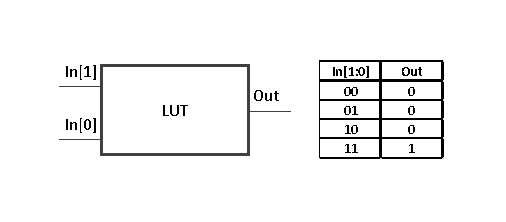
\includegraphics[scale=1.5]{img/lutExample.pdf}
			\caption{LUT Example}
			\label{fig:lutExample}
			\end{figure}

		\begin{table}[!h]
		\centering
		\caption{Sumário de utilização da FPGA}
		\label{tab:fpgaUtilizationSumary}
			\begin{tabular}{lccc}
			\multicolumn{4}{c}{\textbf{Utilização de Slices Lógicos}}                                                                                                    \\ \cline{2-4} 
			\multicolumn{1}{l|}{}                                    & \multicolumn{1}{l|}{Usado} & \multicolumn{1}{l|}{Disponível} & \multicolumn{1}{l|}{Utilização}  \\ \hline
			\multicolumn{1}{|l|}{Quantidade de Registradores Slices} & \multicolumn{1}{c|}{2173}  & \multicolumn{1}{c|}{301440}     & \multicolumn{1}{c|}{0,72\%}      \\ \hline
			\multicolumn{1}{|l|}{Quantidade de LUTs Slice}           & \multicolumn{1}{c|}{1645}  & \multicolumn{1}{c|}{150720}     & \multicolumn{1}{c|}{1,09\%}      \\ \hline
			                                                         &                            &                                 &                                  \\
			\multicolumn{4}{c}{\textbf{Distribuição dos Slices Lógicos}}                                                                                                   \\ \cline{2-4} 
			\multicolumn{1}{l|}{}                                       & \multicolumn{1}{l|}{Usado} & \multicolumn{1}{l|}{Disponível} & \multicolumn{1}{l|}{Utilização} \\ \hline
			\multicolumn{1}{|l|}{Número de Flip Flops não utilizados}   & \multicolumn{1}{c|}{1308} & \multicolumn{1}{c|}{3481}      & \multicolumn{1}{c|}{37,58\%}     \\ \hline
			\multicolumn{1}{|l|}{Número de LUTS não utulizadas}         & \multicolumn{1}{c|}{1836} & \multicolumn{1}{c|}{3481}      & \multicolumn{1}{c|}{52,74\%}     \\ \hline
			\multicolumn{1}{|l|}{Número de pares LUT-FF utilizados}     & \multicolumn{1}{c|}{337}  & \multicolumn{1}{c|}{3481}      & \multicolumn{1}{c|}{9,68\%}      \\ \hline
			                                                            &                           &                                &                                  \\
			% \multicolumn{4}{c}{\textbf{Specific Feature Utilization}}                                                                                               \\ \cline{2-4} 
			% \multicolumn{1}{l|}{}                                   & \multicolumn{1}{l|}{Used} & \multicolumn{1}{l|}{Available} & \multicolumn{1}{l|}{Utilization} \\ \hline
			% \multicolumn{1}{|l|}{Number of BUFG/BUFGCTRLs}          & \multicolumn{1}{c|}{2}    & \multicolumn{1}{c|}{32}        & \multicolumn{1}{c|}{6,25\%}      \\ \hline
			% \multicolumn{1}{|l|}{Number of DSP48E1s}                & \multicolumn{1}{c|}{10}   & \multicolumn{1}{c|}{768}       & \multicolumn{1}{c|}{1,30\%}      \\ \hline
			\end{tabular}
		\end{table}

		Em \cite{Bhavanam1} e \cite{Bhavanam2} são sintetizados detectores DTMF. Nestes trabalhos são informados dados como área e potência do hardware
		sintetizado.


		% \newpage

		\section{Análise dos tempos de processamento}
			Para o \textit{Tone Detector} existem dois tempos que são cruciais para o processamento, 
			o primeiro é o tempo que o \textit{Command Handler} leva para receber o comando e escrevê-lo na memória, e
			o segundo é o intervalo de tempo em que o 
			\textit{Signal Processor} leva para processar um canal.

			Depois de o comando ser recebido, o \textit{Command Handler} faz a requisição para escrever na memória os parâmetros da detecção. Com a autorização
			para que a escrita seja feita, leva-se dez ciclos de clock para que a ação seja concluída, para o recebimento deste comando leva-se também dez ciclos,
			totalizando vinte ciclos de clock para o recebimento e escrita na memória, do comando.
			Para o \textit{Signal Processor}, o pior de caso de execução, ou seja, a situação em que leva-se mais tempo para processar um canal, 
			gasta-se quarenta e cinco ciclos de clock, sendo
			vinte e seis ciclos para ler a região de memória do canal, cinco ciclos de processamento, 
			treze para a escrita na memória e um para a mudança para o próximo canal.
			
			Como a frequência do clock é $80 MHz$, o perído é $12,5 ns$, assim temos que no total, o \textit{Command Handler} gasta $250ns$ para escrever
			os parâmetros na memória. O \textit{Signal Processor} leva $562,5 ns$ por canal, no pior caso de execução. 
			Como a taxa de atualização dos frames é $8KHz$, ou seja, o \textit{Tone Detector} tem uma janela
			de processamento de $125 \mu s$ para processar todos os canais.

			Com as informações de tempo de escrita dos parâmetros na memória, e dos tempos de processamento do \textit{Signal Processor}, podemos extrair 
			a informação de quantidade máxima de canais possíveis de serem processados, sobre duas situações distintas: Não havendo escrita de comandos na memória;
			Escrita de vinte comandos na memória. Em ambas as situações, todos os canais estão processando, e no pior caso de execução.

			Na primeira situação, temos que a janela de processamento está totalmente disponível para o \textit{Signal Processor}, ou seja, a quantidade máxima
			de canais possíveis de processar é:

				\begin{align}
					n_{max} = \frac{\textit{Janela de processamento}}{\textit{Tempo de processamento}} =\frac{125\mu s}{562,5 ns} = 222 \textit{ canais}
				\end{align}

			Na segunda situação, com a escrita de vinte comandos na memória, temos:

			\begin{align}
					n_{max} &= \frac{\textit{(Janela de processamento)}-20.\textit{(Tempo de escrita do comando)} }{\textit{Tempo de processamento}} \\
						&=\frac{125\mu s - 20.250ns }{562,5 ns} \\
						&= 213 \textit{ canais}
			\end{align}

			De maneira geral, o número máximo de canais possíveis de serem processados é:


			\begin{align}
					n_{max} &= \frac{\textit{(Janela de processamento)}-n_{comandos}.\textit{(Tempo de escrita por comando)} }{\textit{Tempo de processamento}}\\
						&=\frac{125\mu s - n_{comandos}.250ns }{562,5 ns}
			\end{align}

			Os valores de quantidade máxima de canais possíveis de serem processados se mostram com valores ótimos, tendo em vista a baixa frequência de clock, 
			o que influi diretamente na potência utilizada pelo \textit{Tone Detector}. Tomando como base o DSP da \textit{Texas Instrument} modelo
			\textit{tms320vc5509a}, que em sua máxima performance, executa uma instrução a cada $5 ns$, implicando que para igualar a performance,
			este DSP teria que fazer todo o processamento em no máximo cento e doze instruções, levando em conta acessos a memória, multiplicações, cálculo do 
			algoritmo de \textit{Goertzel}, etc. O cálculo da quantidade de instruções necessárias é feito baseado no tempo gasto pelo \textit{Signal Processor}
			para processar um canal, que é $562,5ns$. 

			O poder de processamento de \textit{Signal Processor} frente ao DSP \textit{tms320vc5509a}, vem do fato de o \textit{Signal Processor}
			ser projetado para uso específico nesse tipo de processamento, além de ser implementado em hardware, que tráz a vantagem
			de a maior parte das operações serem efetuadas em paralelo.


		\subsection{Comparação de desempenho temporal}
			Para métrica de comparação, foi utilizado o \textit{Aplication Note}, da \textit{Silicon Labs}, \cite{siliconLabs1}, no qual foram 
			realizados testes de desempenho em três testes: Projetos de filtros FIR; Algoritmos de Goertzel para
			detecção DTMF; Algoritmo da FFT. Para comparação usamos os resultados obtidos da utilização do algoritmo de Goertzel para a detecção DTMF.


			% Para métrica de comparação, foi utilizado o documento REFERENCIA  %% referenciar o site
			% presente no site da \textit{Silicon Labs}, no qual faz testes de performance em 3 testes: Projetos de filtros FIR; Algoritmos de Goertzel para
			% detecção DTMF; Algoritmo da FFT. Para comparação usamos os resultados obtidos da utilização do algoritmo de Goertzel para a detecção DTMF.

			Sinais DTMF(\textit{Dual-Tone Multi-Frequency}), são sinais compostos pela soma de sinais com baixa frequência e outro com alta frequência,
			como pode ser visto na Figura \ref{fig:dtmfDigits}.
			Na telefonia são utilizados	para sinalizar os dígitos do teclado numérico. 

				\begin{figure}[!h]
				\centering 
				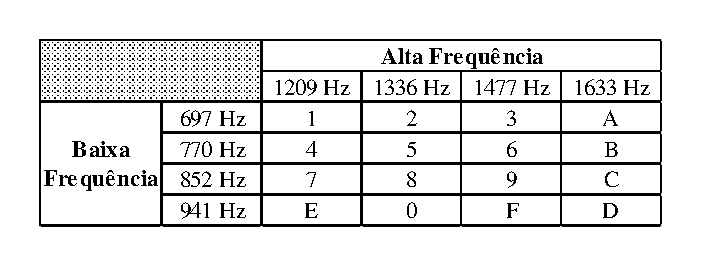
\includegraphics[scale=1]{img/DTMF.pdf}
				\caption{Dígitos DTMF}
				\label{fig:dtmfDigits}
				\end{figure}

			Na detecção de dígitos DTMF implementada em \cite{siliconLabs1}, assim como nesse trabalho, o algoritmo de Goertzel foi utilizado, mas na detecção 
			de dígitos DTMF, existem 
			oito frequências que têm que ser verificadas, diferente da detecção deste trabalho, que processa duas frequências para cada frame de áudio.

			No trabalho da \textit{Silicon Labs}, \cite{siliconLabs1}, foi utilizado um DSP da família C8051F12x, que tem uma frequência máxima de $25 MHz$. 
			São apresentados resultados para o processamento das oito frequências presentes na detecção DTMF
			em diferentes níveis de desempenho do DSP, escolhendo o caso de maior desempenho, que é na utilização de instruções MAC com implementação de 
			noventa e oito MIPS(milhões de instruções por segundo). A comparação foi realizada 
			somente sob o segmento de código responsável pelo processamento.


			Para comparação direta com os resultados do documento referenciado, fizemos uma redução no clock do \textit{Tone Detector} para $25 MHz$, assim tendo
			como período $40 ns$, e para o processamento das oito frequências, faremos a utilização de quatro canais. 
			No \textit{Tone Detector} são gastos 42 ciclos de clock para o cálculo do primeiro passo
			do algoritmo de Goertzel, incluindo leitura e escrita na memória, e três ciclos
			para o cálculo da segunda etapa, a potência do sinal, que inclui a fase de verificação dos resultados também, portanto, são 
			quarenta e cinco ciclos
			para processar dois frequências, assim, para oito temos um total de cento e sessenta e oito ciclos para o cálculo de Goertzel e 
			doze para o cálculo da da potência. 
			Os resultados do cálculo do algoritmo de Goertzel, dos dois trabalhos encontram-se na Tabela \ref{tab:resultComparison}.		


				\begin{table}[!h]
				\centering
				\caption{Comparação dos resultados}
				\label{tab:resultComparison}
				\begin{tabular}{|c|c|c|c|c|c|c|}
				\hline
				\multirow{2}{*}{\textbf{}}                                                                    & \multicolumn{2}{c|}{\textbf{C8051F12x}}                                 & \multicolumn{2}{c|}{\textbf{Tone Detector}}                             & \multicolumn{2}{c|}{\textbf{\% de Redução}}                               \\ \cline{2-7} 
				                                                                                              & \begin{tabular}[c]{@{}c@{}}Ciclos \\ de \\ clock\end{tabular} & $\mu s$ & \begin{tabular}[c]{@{}c@{}}Ciclos \\ de \\ clock\end{tabular} & $\mu s$ & \begin{tabular}[c]{@{}c@{}}Ciclos\\ de Clock\end{tabular} & Tempo \\ \hline
				\textbf{Gortzel}                                                                              & 1018                                                          & 10,4    & 168                                                           & 6,72    & 83,49\%                                                   & 35,39\% \\ \hline
				\textbf{Potência}                                                                             & 1743                                                          & 17,8    & 12                                                            & 0,48    & 99,31\%                                                   & 97,30\% \\ \hline
				\textbf{\begin{tabular}[c]{@{}c@{}}Goertzel \\ +\\  Potência\end{tabular}}                    & 2761                                                          & 28,2    & 180                                                           & 7,2     & 93,48\%                                                   & 74,47\% \\ \hline
				\textbf{\begin{tabular}[c]{@{}c@{}}Tempo total\\  para 200 samples\\ de entrada\end{tabular}} & 205000                                                        & 2095    & 33612                                                         & 1344    & 83,60\%                                                   & 35,85\% \\ \hline
				\end{tabular}
				\end{table}

			Analisando a Tabela \ref{tab:resultComparison} podemos constatar que o \textit{Tone Detector} obteve grande desempenho frente à implementação referenciada. Para um processamento
			com duzentas amostras por frame, obtivemos uma grande redução nos ciclos de clock necessários para realizar a mesma tarefa, tendo uma redução de 
			$83,60\%$, alcançando uma redução de $751 \mu s$, equivalendo a $35,85 \%$ em relação à aplicação da \textit{Silicon Labs}. 




		\section{Resultado das simulações}
			As simulações foram realizadas, através do bloco de unidade de testes, descrito na Seção \ref{sec:testUnitySection}, para isto, são inseridos, 
			por canal, o comando contendo os parâmetros e o áudio relativo a este comando.
			O resultado das simulações é obtido através da análise das mensagens que o \textit{Tone Detector} retorna, são três tipos, mensagens de detecção,
			\textit{timeout} de pulsos e \textit{timeourt} de pausas. Para a análise das mensagens, foram gerados áudios com essas três características.

			Do universo de áudios gerados, na média $50\%$ correspondem a parcela de sinais que foram gerados com \textit{timeout}, sendo $25\%$ de pulsos e
			$25\%$ de pausas. Os $50\%$ restantes são sinais em que suas características estão descritas de acordo com os parâmetros passados.

			Para fazer a análise foram gerados dois mil áudios, dentre estes novecentos e noventa e quatro correspondem a áudios corretos, 
			quinhentos e doze são áudios com \textit{timeout} de pulso e
			quatrocentos e noventa e quatro são correspondem a \textit{timeout} de pausa. Para fazer a simulação do processamento de todos os áudios,
			levou-se $25h20m$, isto para simular um tempo de $6m40s$. 

			O resultado da análise da simulação do \textit{Tone Detector} nos mostra que foi obtido uma taxa de acerto de $100\%$, isto é,
			todos os áudios sem \textit{timeout} foram detectados corretamente, assim como todos o áudios com \textit{timeout} de pulso ou de pausa tiveram
			esta falha detectada.
			Essa taxa de acerto devido ao fato de que o processamento do \textit{Tone Detector} não é probabilístico, ou seja, quando um áudio tem seu processamento
			iniciado só existe como possibilidade, este ser detectado, ou não.








	


\end{document}
